\documentclass[a4paper, 11pt]{article}
\usepackage[UTF8]{ctex}
\usepackage{amsmath}
\usepackage{graphicx}
\usepackage{geometry}
\usepackage{listings}
\geometry{scale=0.8}
\usepackage{hyperref}
\usepackage{enumerate}
\usepackage{color}
\linespread{1.5}

\title{
\normalfont \normalsize
\textsc{School of Data and Computer Science, Sun Yat-sen University} \\ [25pt] %textsc small capital letters
\rule{\textwidth}{0.5pt} \\[0.4cm] % Thin top horizontal rule
\huge  T03 Planning and Uncertainty\\ % The assignment title
\rule{\textwidth}{2pt} \\[0.5cm] % Thick bottom horizontal rule
\author{16337110 匡乾, 16337111 赖若潘}
\date{\normalsize\today}
}

\begin{document}
\maketitle
\tableofcontents
\newpage
\section{Q1}
\begin{enumerate}[(a)]
  \item
  % $(at(o,l1,s) \bigwedge \lnot at(o,l2,s)) \bigvee(at(o,l2,s) \bigwedge \lnot at(o,l1,s))$
   $\forall s\forall l_1\forall l_2(at(o,l_1,s) \bigwedge at(o,l_2,s) \Rightarrow l_1 = l_2)$
  \item
  $s_0$: $\lnot lightOn(s_0) \bigwedge at(shakey,r_1,s_0) \bigwedge at(b1,r_2,s_0) \bigwedge at(b2,r_3,s_0)$\\
  goal situation: $\exists s,lightOn(\phi (s))$

  \item
$walkTo(loc_1,loc_2)$\\
	precondition: $at(shakey,loc_1,s)$\\
	effect: $at(shakey,loc_2,s) \bigwedge \lnot at(shakey,loc_1,s)$\\

$push(box,loc_1,loc_2)$\\
	precondition: $at(shakey,loc_1,s) \bigwedge at(box,loc_1,s)$\\
	effect: $at(box,loc_2,s) \bigwedge \lnot at(box,loc_1,s)$\\

$turnOn$\\
	precondition: $at(b_1,r_1,s) \bigwedge at(b_2,r_2,s) \bigwedge at(shakey,r_1,s)$\\
	effect: $lightOn(s)$

  \item
  $1.(\lnot lightOn(s_0))$\\
  $2.(at(shakey,r_1,s_0))$\\
  $3.(at(b1,r_2,s_0))$\\
  $4.(at(b2,r_3,s_0))$\\
  $5.(at(shakey,loc_1,s),\lnot at(shakey,loc_1,do(walkTo(loc_1,loc_2),s)))$\\
  $6.(at(shakey,loc_1,s),at(shakey,loc_2,do(walkTo(loc_1,loc_2),s)))$\\
  $7.(at(shakey,loc_1,s),at(box,loc_1,s),at(box,loc_2,do(push(box,loc_1,loc_2),s)))$\\
  $8.(at(shakey,loc_1,s),at(box,loc_1,s),\lnot at(box,loc_1,do(push(box,loc_1,loc_2),s)))$\\
  $9.(at(b_1,r_1,s),at(b_2,r_2,s),at(shakey,r_1,s),lightOn(do(turnOn),s))$\\
  $10.(\lnot lightOn(z),ans(z))$\\
  And by resolution, we can get $ans(z,s_0)$\\
  $z = do(turnOn,do(walkTo(r_2,r_1),do(push(b_1,r_2,r_1),do(walkTo(r_3,r_2),\\
  do(push(b_2,r_3,r_2),do(walkTo(r_2,r_3),do(walkTo(r_1,r_2))))))))$\\

\end{enumerate}


\section{Q2}
\begin{enumerate}[(a)]
  \item
  \begin{itemize}
    \item actions:
      \begin{itemize}
        \item move(x, a, b):\\
        Pre:\{on(x, a), clear(x), clear(b), smaller(x, b)\}\\
        Adds:\{on(x, b), clear(a)\}\\
        Dels:\{on(x, a), clear(b)\}
        \item moveTwo(x, y, a, b):\\
            Pre:\{on(x, y), on(y, a), clear(x), clear(b), smaller(y, b)\}\\
            Adds:\{on(y, b), clear(a)\}\\
            Dels:\{on(y, a), clear(b)\}
      \end{itemize}

    \item initial KB:
    $\{ on(d_{1}, d_{2}), on(d_{2}, d_{3}), on(d_{3}, p_{1}), clear(d_{1}), clear(p_{2}), clear(p_{3}) \}$
    \item goal:
    $\{ on(d_{1}, d_{2}), on(d_{2}, d_{3}), on(d_{3}, p_{3}), clear(d_{1}), clear(p_{1}), clear(p_{2}) \}$
  \end{itemize}
  \item
  Reachability Analysis:\\
  $S_{0} = \{ \textcolor{red}{on(d_{1}, d_{2}), on(d_{2}, d_{3}), clear(d_{1}), clear(p_{2}), } on(d_{3}, p_{1}), clear(p_{3})\}$\\
  $A_{0} = \{ [on(d_{1}, d_{2}), clear(d_{1}), clear(p_{2}), smaller(d_{1}, p_{2})]move(d_{1},d_{2},p_{2})[on(d_{1}, p_{2}), clear(d_{2})],$\\
       $[on(d_{1}, d_{2}), clear(d_{1}), clear(p_{3}), smaller(d_{1}, p_{3})]move(d_{1},d_{2},p_{3})[on(d_{1}, p_{3}), clear(d_{2})],$\\
       $[on(d_{1}, d_{2}), on(d_{2}, d_{3}), clear(d_{1}), clear(p_{2}), smaller(d_{2},p_{2})]move(d_{1},d_{2},d_{3},p_{2})[on(d_{2}, p_{2}), clear(d_{3})]$\\
       $[on(d_{1}, d_{2}), on(d_{2}, d_{3}), clear(d_{1}), clear(p_{3}), smaller(d_{2},p_{3})]move(d_{1},d_{2},d_{3},p_{3})[on(d_{2}, p_{3}), clear(d_{3})]\}$\\
  $S_{1} = \{ \textcolor{red}{on(d_{1}, d_{2}), on(d_{2}, d_{3}), clear(d_{1}), clear(p_{2}), } on(d_{3}, p_{1}), clear(p_{3}),on(d_{1}, p_{2}), $\\
              $on(d_{1}, p_{3}), clear(d_{2}), on(d_{2}, p_{2}), on(d_{2}, p_{3}), clear(d_{3})\}$\\
  $A_{1} = \{ [on(d_{3},p_{1}), clear(d_{3}), clear(p_{3}), smaller(d_{3}, p_{3})]move(d_{3},p_{1},p_{3})[on(d_{3}, p_{3}), clear(p_{1})]$
            $ \cdots \}$\\
  $S_{2} = \{ \textcolor{red}{on(d_{1}, d_{2}), on(d_{2}, d_{3}), clear(d_{1}), clear(p_{2}), on(d_{3},p_{3}), clear(p_{1}), } on(d_{3}, p_{1}), $ \\
              $clear(p_{3}),on(d_{1}, p_{2}), on(d_{1}, p_{3}), clear(d_{2}), on(d_{2}, p_{2}), on(d_{2}, p_{3}), clear(d_{3}) \cdots\}$
  \\因为goal$\ \notin S_{1}$, goal$\ \in S_{2}$, 所以停止, 接下来计算启发式函数的值。\\
$CountAction(G,S_{2}):$\\
$G_{P} = \{ on(d_{1},d_{2}),on(d_{2},d_{3}),clear(d_{1}),clear(p_{2})\}$\\
$G_{N} = \{ on(d_{3},p_{3}),clear(p_{1})\}$\\
$A = \{ move(d_{3},p_{1},p_{3})\}$\\
$G_{1} = G_{P} \cup Pre(A) = \{ on(d_{1},d_{2}),on(d_{2},d_{3}),clear(d_{1}),clear(p_{2}), on(d_{3},p_{1}), clear(d_{3}), clear(p_{3})\}$\\
$return\ 1 + CountAction(G_{1},S_{1})$\\

$CountAction(G_{1},S_{1}):$\\
$G_{P} = \{ on(d_{1},d_{2}),on(d_{2},d_{3}),clear(d_{1}),clear(p_{2})\}$\\
$G_{N} = \{ on(d_{3},p_{1}), clear(d_{3}), clear(p_{3})\}$\\
$A = \{ move(d_{1},d_{2},d_{3},p_{2})\}$\\
$G_{2} = G_{P} \cup Pre(A) = \{ on(d_{1},d_{2}),on(d_{2},d_{3}),clear(d_{1}),clear(p_{2}) \}$\\
$return\ 1 + CountAction(G_{2},S_{0})$\\

$CountAction(G_{2},S_{0}) = 0$\\
综上:$CountAction(G,S_{2}) = 1+1+0 = 2$
\end{enumerate}

\section{Q3}
\begin{enumerate}
  \item
    \begin{enumerate}[(a)]
      \item see the Figure \ref{Q3fig1}.
      \begin{figure}[htbp]
        \centering
        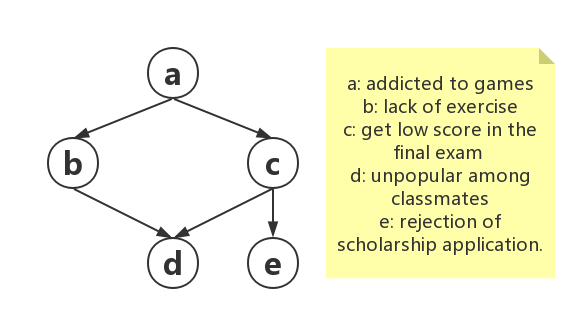
\includegraphics[width=15cm]{pic/1}
        \caption{Q3 1(a)}
        \label{Q3fig1}
      \end{figure}
      \item
      e is independent of a,b,d, given c.

      b is independent of c, given a.

      d is independent of a, given b and c.

      \item
      设节点a的因子为$f_{1}(A)$, 节点b因子为$f_{2}(A,B)$, 节点c因子为
      $f_{3}(A,C)$, 节点d因子为$f_{4}(B,C,D)$, 节点e因子为$f_{5}(C,E)$,由题目已知条件得到表\ref{Q3T1}\\

      \begin{table}[htbp]
        \centering
        \begin{tabular}{|l|c|}
          \hline
          $a$&0.2\\
          \hline
          $\lnot a$&0.8\\
          \hline
        \end{tabular}
        \begin{tabular}{|l|c|}
          \hline
          $ab$&0.7\\
          \hline
          $a\lnot b$&0.3\\
          \hline
          $\lnot ab$&0.2\\
          \hline
          $\lnot a\lnot b$&0.8\\
          \hline
        \end{tabular}
        \begin{tabular}{|l|c|}
          \hline
          $ac$&0.2\\
          \hline
          $a\lnot c$&0.8\\
          \hline
          $\lnot ac$&0.05\\
          \hline
          $\lnot a\lnot c$&0.95\\
          \hline
        \end{tabular}
        \begin{tabular}{|l|c|}
          \hline
          $bcd$&0.8\\
          \hline
          $bc\lnot d$&0.2\\
          \hline
          $b\lnot cd$&0.7\\
          \hline
          $b\lnot c\lnot d$&0.3\\
          \hline
          $\lnot bcd$&0.7\\
          \hline
          $\lnot bc\lnot d$&0.3\\
          \hline
          $\lnot b \lnot cd$&0.05\\
          \hline
          $\lnot b \lnot c \lnot d$&0.95\\
          \hline
        \end{tabular}
        \begin{tabular}{|l|c|}
          \hline
          $ce$&0.7\\
          \hline
          $c\lnot e$&0.3\\
          \hline
          $\lnot ce$&0.6\\
          \hline
          $\lnot c\lnot e$&0.4\\
          \hline
        \end{tabular}
        \caption{$f_{1}(A), f_{2}(A,B),f_{3}(A,C),f_{4}(B,C,D),f_{5}(C,E)$}
        \label{Q3T1}
      \end{table}

      要计算$P(A,B,C|\lnot d,e)$,因证据变量为$D=\lnot d, E=e$,故可以得到$f_4(B,C,D=\lnot d)=f_6(B,C)$以及$f_5(C,E=e)=f_7(C)$,见表\ref{Q3T6}。
      \begin{table}[htbp]
        \centering
        \begin{tabular}{|l|c|}
          \hline
          $bc$&0.2\\
          \hline
          $b\lnot c$&0.3\\
          \hline
          $\lnot bc$&0.3\\
          \hline
          $\lnot b\lnot c$&0.95\\
          \hline
        \end{tabular}
        \begin{tabular}{|l|c|}
          \hline
          $c$&0.7\\
          \hline
          $\lnot c$&0.6\\
          \hline
        \end{tabular}
        \caption{$f_6(B,C),f_7(C)$}
        \label{Q3T6}
      \end{table}

    经过计算并归一化后我们可以得到表\ref{Q3T2}
    % \begin{align*}
    %   & = \sum_{A,B,C}P(A,B,C,-d,e)\\
    %   & =\sum_{A,B,C}P(A)P(B|A)P(C|A)P(-d|B,C)P(e|C)\\
    %   & =\sum_{A}P(A)\sum_{B}P(B|A)\sum_{C}P(C|A)P(e|C)P(-d|B,C)\\
    %   & =P(a)\sum_{B}P(B|a)\sum_{C}P(C|a)P(e|C)P(d|B,C)\\
    %   & +P(-a)\sum_{B}P(B|-a)\sum_{C}P(C|-a)P(e|C)P(d|B,C)\\
    %   & =P(a)P(b|a)\sum_{C}P(C|a)P(e|C)P(d|b,C)\\
    %   & +P(a)P(-b|a)\sum_{C}P(C|a)P(e|C)P(d|-b,C)\\
    %   & +P(-a)P(b|-a)\sum_{C}P(C|-a)P(e|C)P(d|b,C)\\
    %   & +P(-a)P(-b|-a)\sum_{C}P(C|-a)P(e|C)P(d|-b,C)\\
    %   & =P(a)P(b|a)P(c|a)P(e|c)P(d|b,c)
    %   +P(a)P(b|a)P(-c|a)P(e|-c)P(d|b,-c)\\
    %   & +P(a)P(-b|a)P(c|a)P(e|c)P(d|-b,c)
    %   +P(a)P(-b|a)P(-c|a)P(e|-c)P(d|-b,-c)\\
    %   & +P(-a)P(b|-a)P(c|-a)P(e|c)P(d|b,c)
    %   +P(-a)P(b|-a)P(-c|-a)P(e|-c)P(d|b,-c)\\
    %   & +P(-a)P(-b|-a)P(c|-a)P(e|c)P(d|-b,c)
    %   +P(-a)P(-b|-a)P(-c|-a)P(e|-c)P(d|-b,-c)\\
    % \end{align*}
    \begin{table}
      \centering
      \begin{tabular}{|l|c|}
        \hline
        $abc$&0.009\\
        \hline
        $ab\lnot c$&0.046\\
        \hline
        $a\lnot bc$&0.006\\
        \hline
        $a\lnot b\lnot c$&0.063\\
        \hline
      \end{tabular}
      \begin{tabular}{|l|c|}
        \hline
        $\lnot abc$&0.003\\
        \hline
        $\lnot ab\lnot c$&0.063\\
        \hline
        $\lnot a\lnot bc$&0.015\\
        \hline
        $\lnot a\lnot b\lnot c$&0.795\\
        \hline
      \end{tabular}
      \caption{$P(A,B,C|\lnot d,e)$}
      \label{Q3T2}
    \end{table}


    \item
    计算$P(a)$,先要计算分布$P(A)$,查询变量为A,证据变量为$D=\lnot d,E=e$,相关变量为A,B,C,D,E。

    首先限制因子,得到$f_{6}(B,C)=f_{4}(B,C,D=\lnot d$,$f_{7}(C)=f_{5}(C,E=e)$,见表\ref{Q3T6}

    设消元顺序为B,C。\\
    B: $f_{2}(A,B),f_{7}(B,C)$\\
    C: $f_{3}(A,C),f_{6}(C)$\\
    消去B,即$f_{8}(A,C)=\sum_B f_{2}(A,B) \times f_{7}(B,C) = f_{2}(A,b)f_{7}(b,C)+f_{2}(A,\lnot b)f_{7}(\lnot b,C)$,见表\ref{Q3T4}\\
    消去C,即$f_{9}(A)=\sum_C f_{3}(A,C) \times f_{6}(C) \times f_{8}(A,C) = f_{3}(A,c)f_{6}(c)f_{8}(A,c)+f_{3}(A,\lnot c)f_{6}(\lnot c)f_{8}(A,\lnot c)$,见表\ref{Q3T4}\\
    故$f_{10}(A)=f_1(A) \times f_9(A)$\\
    最后对$f_{11}(A)$归一化,得到$f_{12}(A)=\alpha f_{11}(A), \alpha = 1/ \sum_A f_{11}(A)$,见表\ref{Q3T4}\\
    因此$P(a|\lnot d,e)=0.124<0.2=P(a)$\\
    因此此时我们更加不倾向于相信学生沉迷于游戏。
    \begin{table}[ht]
      \centering
      \begin{tabular}{|l|c|}
        \hline
        $ac$&0.23\\
        \hline
        $a\lnot c$&0.495\\
        \hline
        $\lnot ac$&0.28\\
        \hline
        $\lnot a\lnot c$&0.82\\
        \hline
      \end{tabular}
      \begin{tabular}{|l|c|}
        \hline
        $a$&0.2698\\
        \hline
        $\lnot a$&0.4772\\
        \hline
      \end{tabular}
      \begin{tabular}{|l|c|}
        \hline
        $a$&0.124\\
        \hline
        $\lnot a$&0.876\\
        \hline
      \end{tabular}
      \caption{$f_8(A,C),f_9(A),f_{11}(A)$}
      \label{Q3T4}
    \end{table}
    \end{enumerate}



  \item
  设节点A的因子为$f_{1}(A)$, 节点B因子为$f_{2}(B)$, 节点C因子为
  $f_{3}(A,B,C)$, 节点D因子为$f_{4}(B,D)$, 节点E因子为$f_{5}(C,E)$,
  节点F因子为$f_{6}(C,F)$,见表(\ref{Q3T2.1})\\
  \begin{table}[ht]
    \centering
    \begin{tabular}{|l|c|}
      \hline
      $a$&0.8\\
      \hline
      $\lnot a$&0.2\\
      \hline
    \end{tabular}
    \begin{tabular}{|l|c|}
      \hline
      $b$&0.2\\
      \hline
      $\lnot b$&0.8\\
      \hline
    \end{tabular}
    \begin{tabular}{|l|c|}
      \hline
      $abc$&0.2\\
      \hline
      $ab\lnot c$&0.8\\
      \hline
      $a\lnot bc$&0.7\\
      \hline
      $a\lnot b \lnot c$&0.3\\
      \hline
      $\lnot abc$&0.8\\
      \hline
      $\lnot ab\lnot c$&0.2\\
      \hline
      $\lnot a \lnot bc$&0.4\\
      \hline
      $\lnot a \lnot b \lnot c$&0.6\\
      \hline
    \end{tabular}
    \begin{tabular}{|l|c|}
      \hline
      $bd$&0.1\\
      \hline
      $b\lnot d$&0.9\\
      \hline
      $\lnot bd$&0.8\\
      \hline
      $\lnot b\lnot d$&0.2\\
      \hline
    \end{tabular}
    \begin{tabular}{|l|c|}
      \hline
      $ce$&0.8\\
      \hline
      $c\lnot e$&0.2\\
      \hline
      $\lnot ce$&0.1\\
      \hline
      $\lnot c\lnot e$&0.9\\
      \hline
    \end{tabular}
    \begin{tabular}{|l|c|}
      \hline
      $cf$&0.2\\
      \hline
      $c\lnot f$&0.8\\
      \hline
      $\lnot cf$&0.8\\
      \hline
      $\lnot c\lnot f$&0.2\\
      \hline
    \end{tabular}
    \caption{$f_{1}(A),f_{2}(B),f_{3}(A,B,C),f_{4}(B,D),f_{5}(C,E),f_{6}(C,F)$}
    \label{Q3T2.1}
  \end{table}

    \begin{enumerate}[(a)]
      \item 计算P(e), 先要计算分布P(E),查询变量为E, 证据变量无,
      那么我们只需考虑查询变量E和E的祖先即可,相关变量为E, C, A, B。\\
      设消元顺序为A,B,C。\\
      $A: f_{1}(A), f_{3}(A,B,C)$\\
      $B: f_{2}(B)$\\
      $C: f_{5}(C,E)$\\
      消去A, 即$f_{7}(B,C) = \sum_{A}f_{1}(A) \times f_{3}(A,B,C) = f_{1}(a)f_{3}(a,B,C) + f_{1}(\lnot a)f_{3}(\lnot a,B,C)$,
      见表(\ref{table:f7,f8,f9})。\\
      $B: f_{2}(B), f_{7}(B,C)$\\
      $C: f_{5}(C,E)$\\
      消去B, 即$f_{8}(C) = \sum_{B}f_{2}(B) \times f_{7}(B,C) = f_{2}(b)f_{7}(b,C) + f_{2}(\lnot b)f_{7}(\lnot b,C)$
      ,见表(\ref{table:f7,f8,f9})。\\
      $C:f_{5}(C,E), f_{8}(C)$\\
      消去C, 即$f_{9}(E) = \sum_{C}f_{5}(C,E) \times f_{8}(C) = f_{5}(c,E)f_{8}(c) + f_{5}(\lnot c,E)f_{8}(\lnot c)$
      ,见表(\ref{table:f7,f8,f9})。\\
      因此$P(e)=P(E=e)=f_{9}(e)=0.5032$
      \begin{table}[!htbp]
        \centering
        \begin{tabular}{|l|c|}
          \hline
          $bc$&0.32\\
          \hline
          $b\lnot c$&0.68\\
          \hline
          $\lnot bc$&0.64\\
          \hline
          $\lnot b\lnot c$&0.36\\
          \hline
        \end{tabular}
        \begin{tabular}{|l|c|}
          \hline
          $c$&0.576\\
          \hline
          $\lnot c$&0.424\\
          \hline
        \end{tabular}
        \begin{tabular}{|l|c|}
          \hline
          $e$&0.5032\\
          \hline
          $\lnot e$&0.4968\\
          \hline
        \end{tabular}
        \caption{$f_{7}(B,C),f_{8}(C),f_{9}(E)$}
        \label{table:f7,f8,f9}
      \end{table}
      \item 计算$P(e|\lnot f)$, 要计算分布$P(E|\lnot f)=\alpha P(E,\lnot F)$,
      相关的变量有E和E的祖先A,B,C还有F(因为证据变量F是相关变量C的后代)。\\
      设消元顺序为A,B,C。\\
      首先限制因子, $f_{10}(C) = f_{6}(C,F=\lnot f)$,见表(\ref{table:f10,f12})\\
      $A: f_{1}(A), f_{3}(A,B,C)$\\
      $B: f_{2}(B)$\\
      $C: f_{5}(C,E),f_{10}(C)$\\
      消去A, 即$\textcolor{red}{f_{7}(B,C) = \sum_{A}f_{1}(A) \times f_{3}(A,B,C)}$, (a)中已经计算出来了,可以直接使用,
      见(a)中表(\ref{table:f7,f8,f9})。\\
      $B: f_{2}(B), f_{7}(B,C)$\\
      $C: f_{5}(C,E),f_{10}(C)$\\
      消去B, 即$\textcolor{red}{f_{8}(C) = \sum_{B}f_{2}(B) \times f_{7}(B,C)}$, (a)中已经计算出来了,可以直接使用,
      见(a)中表(\ref{table:f7,f8,f9})。\\
      $C: f_{5}(C,E),f_{10}(C),f_{8}(C)$\\
      消去C, 即$f_{11}(E) = \sum_{C}f_{5}(C,E)\times f_{10}(C)\times f_{8}(C)$\\
      最后对$f_{11}(E)$归一化, $f_{12}(E) = \alpha f_{11}(E),\ \alpha = 1/\sum_{E}f_{11}(E)$
      ,见表(\ref{table:f10,f12})。
      \\因此$P(e|\lnot f) = P(E=e|\lnot f) = f_{12}(e) = 0.6912$
      \begin{table}[!ht]
        \centering
        \begin{tabular}{|l|c|}
          \hline
          $c$&0.8\\
          \hline
          $\lnot c$&0.2\\
          \hline
        \end{tabular}
        \begin{tabular}{|l|c|}
          \hline
          $e$&0.6912\\
          \hline
          $\lnot e$&0.3088\\
          \hline
        \end{tabular}
        \caption{$f_{10}(C),f_{12}(E)$}
        \label{table:f10,f12}
      \end{table}
    \end{enumerate}
\end{enumerate}



%\clearpage
%\bibliography{E:/Papers/LiuLab}
%\bibliographystyle{apalike}
\end{document}


%%% Local Variables:
%%% mode: latex
%%% TeX-master: t
%%% End:
